\documentclass{article}
\title{Integrated data analysis for early warning of lung failure \\ \large{Geisinger Health Collider Project: Stage 1}}
\author{The Outliers: Rebecca Barter and Shamindra Shrotriya}
\usepackage{amsmath}
\usepackage{a4wide}
\usepackage{amscd}
\usepackage[tableposition=top]{caption}
\usepackage{ifthen}
\usepackage[pdftex]{graphicx,epsfig,pict2e}
\usepackage{setspace}
\usepackage{float}
\usepackage{amsfonts}
\usepackage[table]{xcolor}
\usepackage{subcaption}
\usepackage[utf8]{inputenc}
\usepackage{cite}
\usepackage{algorithm} 
\usepackage{algpseudocode}
\usepackage{lscape}
\usepackage{hyperref}
\usepackage{rotating}
\usepackage{color}
\usepackage{bbm}

\setlength\parindent{0pt}

\begin{document}
\maketitle

\section{Introduction}

Chronic obstructive pulmonary disease (COPD) is a major cause of mortality worldwide, however many of those with COPD remain undiagnosed. Individuals with undiagnosed COPD typically experience related adverse health effects resulting in increased utilization of health care services. One of the primary reasons for hospitalizations amongst undiagnosed COPD patients is pneumonia; amongst patients with a secondary diagnosis of acute exacerbation of Chronic obstructive pulmonary disease (COPD), pneumonia was the primary reason for hospitalization for 22.3 percent of admissions. For this project, our aim is to develop methods capable of effectively predicting cases of undiagnosed COPD amongst those whose primary reason for hospitalization was pneumonia. Most existing algorithmic approaches to this prediction problem focus only on utilizing clinical information, however we aim to incorporate external data sources primarily related to relevant socioeconomic factors that are not captured by the clinical records using a process called ``data blending''. 

%\section{Introduction}
%
%Chronic obstructive pulmonary disease (COPD) is a major cause of mortality worldwide~\cite{lozano_global_2012}, with approximately 12 million adults in the U.S. having been diagnosed with COPD. Crucially, however, it is estimated that a further 12 million adults in the U.S. have undiagnosed COPD~\cite{nih_chronic_2010}. One of the most common causes of COPD is cigarette smoking, however as many of 10-20\% of COPD patients have never smoked and only a fraction of smokers develop COPD. These insights are suggestive of alternate risk factors such as genetic and environmental. With this in mind, our goal is to ``blend'' external environmental data with the clinical data using a novel blending approach with the hopes of increasing our ability to predict undiagnosed COPD amongst those hospitalized with pneumonia. . 


\section{Data}

The clinical data we will use in this project will include data collected from 
patients who are a part of the Geisinger Health System. The dataset consists of 
data from a total population of 88,000, among whom, 1,033 have 
a ``discharge diagnosis of COPD''. The clinical dataset contains approximately 
80 unique variables sourced primarily from medical records with a few variables 
sourced from billing records. We will be comparing two sub-populations

\begin{enumerate}
\item The COPD subpopulation: all patients who have been diagnosed with COPD.
\item The non-COPD pneumonia subpopulation: those who are diagnosed at a single 
visit with pneumonia and subsequently recover. We do not include in this 
subpopulation those who are re-admitted at multiple visits with pneumonia, 
since this may be indicative of undiagnosed COPD.
\end{enumerate}

\subsection{External data sources}

As a major focus of this project is to blend external data sources with the clinical data described above. This task is poised with a number of challenges. Firstly to ensure that the external data was suitable for the task at hand, we aimed to ensure that a number of requirements were met:
\begin{itemize}
\item {\bf Publicly available}: We require that the data be ``publicly available'', which, here, means that the data is stored in a digital format on the internet on secure servers which are accessible globally. 
\item {\bf Data is obtained from a trustworthy source}: The data source must be trustworthy; that is, the sourced data was created or collected by a legitimate organization, such as government departments. 
\item {\bf The data must be de-identified}: The data much contain no Personally Identifiable Information (PII) in order to ensure that the privacy of all individuals whose information is stored in the dataset is de-identified (that is it does not contain information such as personal address, name and date-of-birth). For data sourced within the Geisinger internal patient database care must be taken to ensure that privacy is protected through discussions with the Geisinger team. 
\item {\bf The data is representative of the population of interest}: Since all Geisinger medical centers are located in Pennsylvania, ideally, we would also like our external data to be from Pennsylvania. Suppose, for example, that we were interested in testing the effect of biomass fuel combustion exposure on COPD, and for our clinical population we imputed the extent of biomass fuel combustion exposure based on data sourced from developing countries in which they use a lot more biofuels. The imputed values from this external data source will be extremely misleading and unlikely to be representative of the amount of biomass fuel combustion on similar people (e.g. similar age, gender, occupation, etc) in developed countries.
\item {\bf The data must contain some variables common to the clinical dataset}: The primary variables based on which we aim to blend data are various combinations of age, gender, zipcode and date. Ideally, to ensure that the blended dataset is as realistic as possible, our external dataset should have, as a bare minimum, each of these variables.
\end{itemize}

Although these requirements seem fairly straighforward; in practice, it turned out to be extremely difficult to find relevant publicly available individual-level data with variables common to the clinical dataset. As a result, we decided to take two alternative approaches. 

First, we first propose to use data collected within the Geisinger health system, but not included in the provided COPD clinical dataset. The primary reason for this approach is three-fold: first of all, as noted above, it is extremely difficult to find individual-level data that is both publicly available AND from a trusted source. Secondly, using data collected by Geisinger ensures that the underlying population mostly matches the population from which the COPD data is drawn, a key concern for the validity of the conclusions drawn from our subsequent analyses. Finally, for the publicly available individual-level data that we could find, it quickly became clear that is is extremely difficult to find adequate variables to match on (where the matching is to match individuals in the external dataset to similar individuals in the clinical dataset). For example, in most cases, the best we could do is matching on age, gender and approximate location, however if we are aiming to impute a variable such as smoking or exposure to biomass fuel combustion, the imputed values is likely to be extremely noisy and not particularly trustworthy (for example, it is highly unlikely that all females, aged 27 who live in Danville, Pennsylvania have the same smoking status; we need more common information between the two datasets).

Our second approach to identifying external data is to use the widely available location-based data (such as weather data, air pollution data or flu trends data), which cannot be imputed at an individual-level. Values of variables imputed from these types of less-granular data sources will be the same for all patients who attend the same Geisinger medical clinic, with the presumption that these patients live within the general proximity of the medical clinic.

The following sections describe the data that we intend to blend (using various methods that will be described below), with the clinical data.

\subsubsection{Smoking data from the Geisinger psychiatric diseases dataset}

As mentioned above, one of the most common causes of COPD is smoking. Although the COPD dataset provided by Geisinger, does not contain the smoking status attribute, the psychiatric diseases dataset does. Assuming that it is not possible to obtain the smoking status of the COPD patients in our dataset, we could use the common attributes of the psychiatric diseases and COPD datasets to predict/impute smoking status. This is an ideal dataset for matching, since (1) the data are sourced from the same population as the patients in the COPD dataset, (2) the data are sourced from a trusted source, and (3) there will be a large number of overlap between the variables. Further, if there are common patients in each dataset, then we could use these patients to devise a supervised learning algorithm which could predict the smoking status of the non-overlapped patients in the COPD dataset (although the method we discuss in our blending section below does not assume any overlap in the two datasets).


\subsubsection{Insurance data from Geisinger health systems}
\textcolor{red}{Write something about (1) the longitudinal flurry of medical claims/hospitalizations that preceeds COPD diagnosis - information that can be obtained from the insurance data (although this could be found in our clinical data too?), and/or (2) the employment information; biofuels inhalation idea}


\subsubsection{Air pollution data from Pennsylvania}
\textcolor{red}{Write about this too!}

\subsubsection{Weather data from Pennsylvania}
\textcolor{red}{And this!}





\section{Data blending}
In this section, we will describe our intended methodology for data blending. Given that we have external data of various different levels of granularity, we will describe each situation individually.


\subsection{Individual-level data blending}

For the datasets for which we can perform individual-level matching, such as the Geisinger psychiatric diseases dataset and the insurance data, we have developed a two-stage blending method. The first stage is a matching stage which involves, for each individual in our clinical dataset, identifying individuals in the external dataset that are most similar in terms of the covariates common to both datasets. In order to effectively blend data sources, there need to be exist common variables using which the datasets can be combined. We propose the following variables to be the minimum required individual-level variables for blending external data sources to the COPD dataset provided: age, gender, zipcode (or hospital zipcode) and the date of patient treatment.

The second stage is an imputation stage which involves imputing or predicting the external variables of interest for the clinical patients by aggregating the values obtained by the matched external individuals. To set up some notation, for observation $i$ in the clinical dataset, we can define a vector of the $p$ observed variables by
$${\bf y}_i = (y_{i1}, ..., y_{ip})^T, ~~~~~ i = 1, ..., n$$

similarly, for the $j$th observation in the external dataset, we can define a vector of the $q$ observed variables by

$${\bf z}_j = (z_{j1}, ..., z_{jq})^T, ~~~~~ j = 1, ..., m$$

Figure~\ref{fig:blend} describes this process for the first individual in the clinical dataset in a general setting.

Suppose that we can reorder these variables so that the first $k \leq \min(p,q)$ variables are common to both datasets, then we can re-write our observations as

$$\text{clinical observation $i$: } ~~{\bf y}_i = (x^c_{i1}, x^c_{i2}, ..., x^c_{ik}, y_{i(k+1)} ..., y_{ip})^T, ~~~~~ i = 1, ..., n$$



$$\text{external observation $j$: }~~{\bf z}_j = (x^e_{j1}, x^e_{j2}, ..., x^e_{jk}, z_{j(k+1)} ..., z_{jq})^T, ~~~~~ j = 1, ..., m$$


where $x_{i1}, ..., x_{ik}$ correspond to the common variables, $y_{j(k+1)}, ..., y_{jp}$ correspond to the variables that are in the clinical dataset but not in the external dataset, and $z_{i(k+1)}, ..., z_{ip}$ correspond to the variables that are in the external dataset but are not in the clinical dataset.

Our goal is to predict the unobserved values of the variables $z_{k+1}, ..., z_q$ for the patients in the clinical dataset. As mentioned above, this process is done in two steps: matching and imputation.





\begin{figure}[H]
\begin{center}
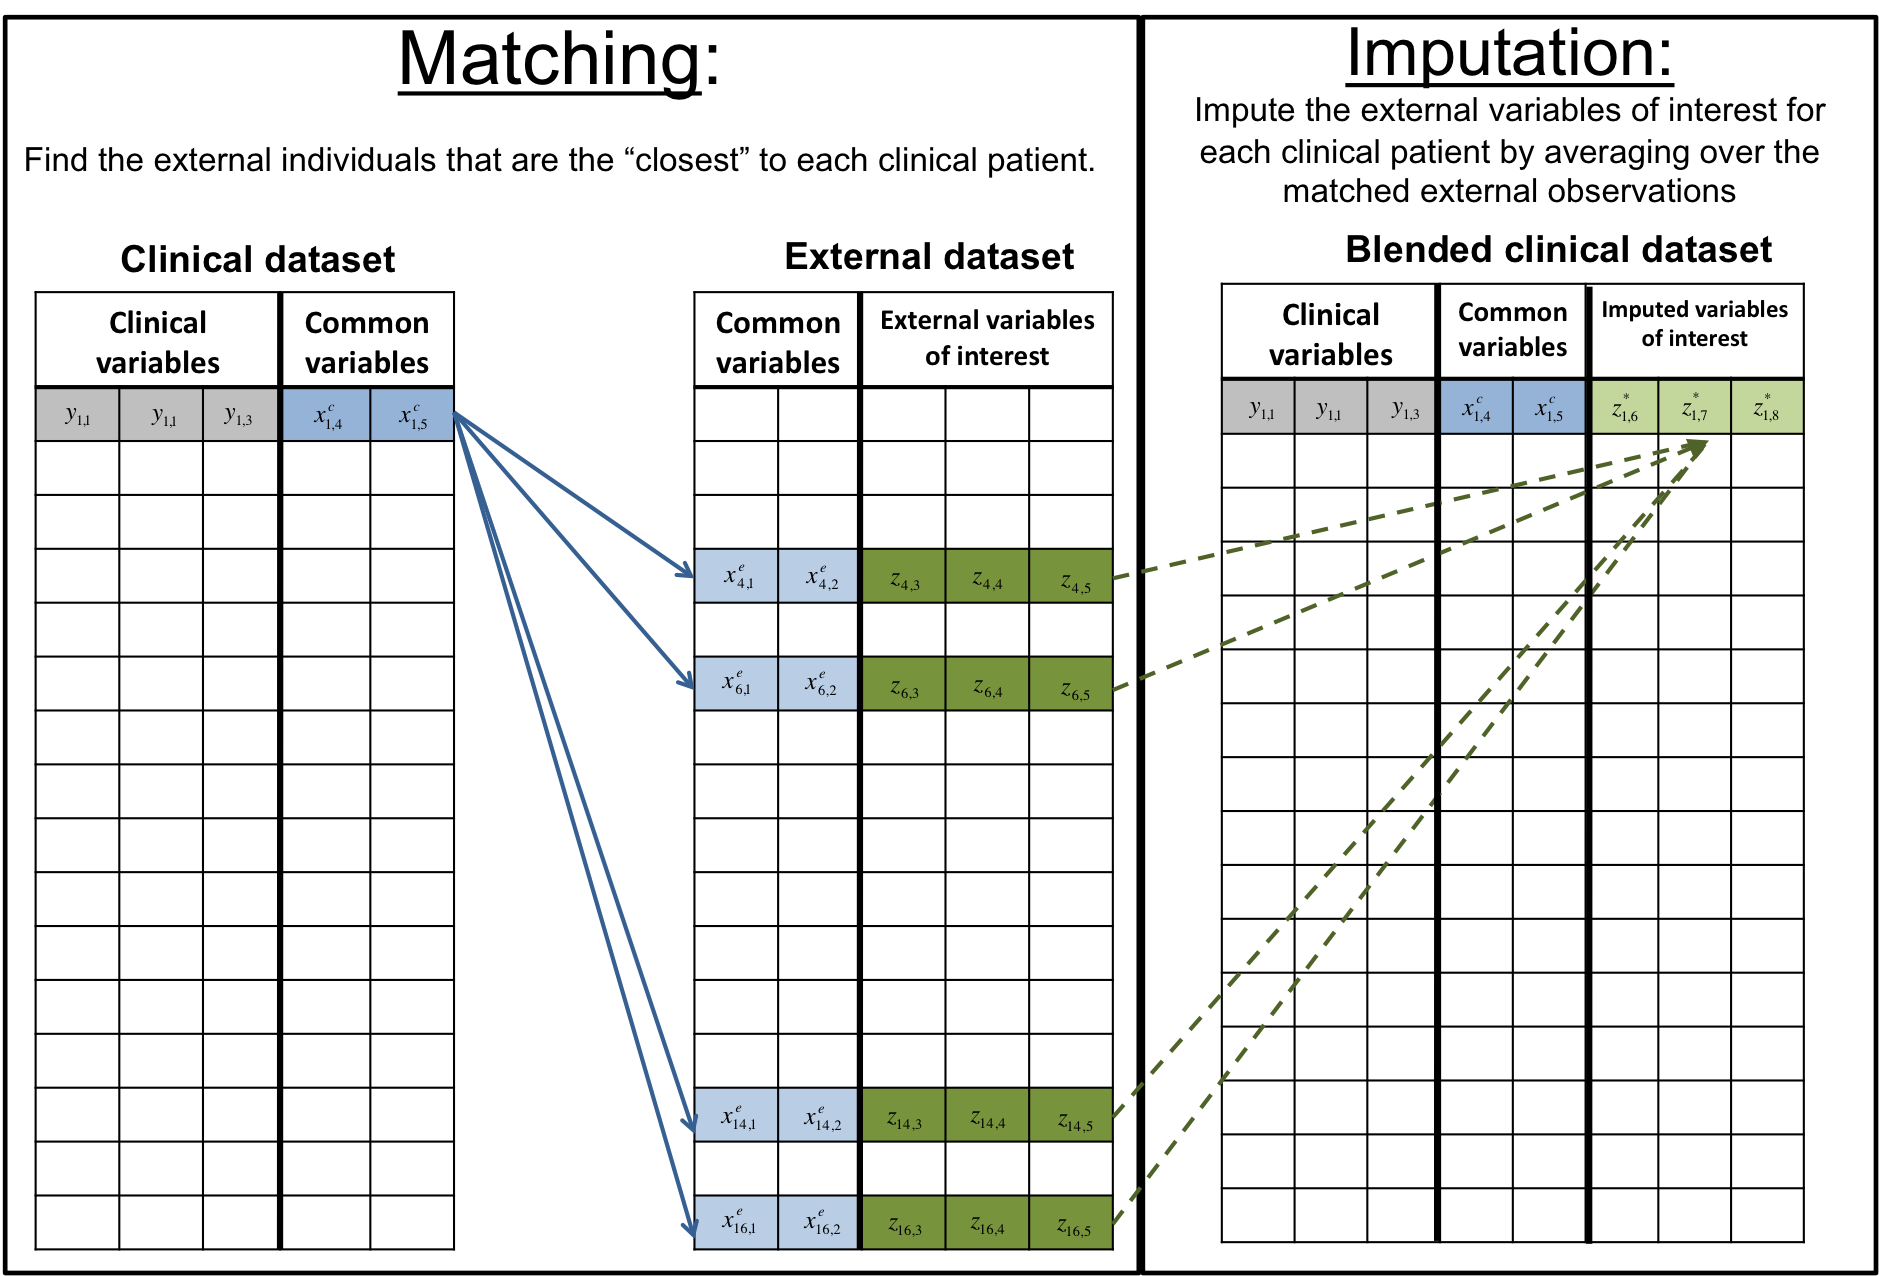
\includegraphics[scale=0.45]{blending.png}
\end{center}
\caption{The data blending process for individual-level blending. For each individual in the clinical dataset, we must identify ``matched'' individuals in the external dataset that are the most similar based on the common variables for both datasets. Then the external variables of interest are imputed for the clinical dataset based on the matched individuals in the external dataset}
\label{fig:blend}
\end{figure}

\subsubsection{The matching step}

To perform matching, we must be able to define a measure of distance between observations in the clinical and external datasets based on the variables that are common to both. We can define the common variables for an observation in the clinical dataset by 
$${\bf x}_i^c = (x_{i1}^c, ..., x_{ik}^c)^T$$
and the common variables for an observation in the external dataset by
$${\bf x}_j^e = (x_{j1}^e, ..., x_{jk}^e)^T$$

The distance between an observation $i$ in the clinical dataset and an observation $j$ in the external dataset, will be defined based on the common variables only, that is
$$d({\bf y}_i, {\bf z}_j) = d({\bf x}_i^c, {\bf x}_j^e)$$

where we can define the distance metric, $d$, in a number of ways, such as the euclidean distance metric:
$$d_{euclidean}({\bf x}_i^c, {\bf x}_j^e) = \sum_{l=1}^k(x_{ij}^c - x_{jl}^e)^2,$$

the Mahalanobis distance metric:
$$d_{mahalanobis}({\bf x}_i^c, {\bf x}_j^e) = \sqrt{({\bf x}_i^c - {\bf x}_j^e)^T S^{-1}({\bf x}_i^c - {\bf x}_j^e)},$$

where $S = cov({\bf x}_i^c, {\bf x}_j^e)$ is the covariance matrix, the correlation metric:

$$d_{corr}({\bf x}_i^c, {\bf x}_j^e) = 1 - corr({\bf x}_i^c, {\bf x}_j^e)$$

or any of the large number of other distance metrics.


For a clinical observation, ${\bf y}_i$, we define a \emph{matched} external observation, to be any ${\bf z}_j$ such that $d({\bf y}_i, {\bf z}_j) = d({\bf x}^c_i, {\bf x}^e_j) < \lambda$ for some threshold, $\lambda$, which could be chosen by a number of methods such as cross-validation to find the value of $\lambda$ that yields the lowest prediction error. 

\subsubsection{The imputation step}


Next, having found matched external observations for each clinical observation, we can impute the values of the external variables of interest that were not present in the clinical dataset. More specifically, suppose that for a clinical observation ${\bf y}_i$, we have $t$ matched external observations, ${\bf z}_1, ..., {\bf z}_t$. We could impute the external observations of interest for the clinical observation by  defining $z^*_{i(k+1)}, ..., z^*_{iq}$ by

$$z^*_{ir} = \frac{1}{t} \sum_{j=1}^t z_{jr}$$

for continuous variables, or by majority vote of the $z_{hr}$ for $h = 1, ..., t$ for categorical variables. Thus, we now have a blended clinical dataset consisting of the blended clinical observations;

$${\bf x}^*_i = (x^c_{i1}, x^c_{i2}, ..., x^c_{ik}, y_{i(k+1)} ..., y_{ip}, z_{i(k+1)}^*, ..., z_{iq}^*)^T$$

which contains all of the original observations in ${\bf x}_i$ along with the imputed observations based on the external matched observations.

An alternative approach which does not involve deciding on a threshold, $\lambda$, for matched observations, is to perform \emph{weighted imputation}. To perform weighted imputation, instead of simply averaging over the external observations most similar to the clinical observation of interest, we calculate a weighted average over all of the external observations, where the external observations ``closest'' to the clinical observation get the highest weights and those furthest get the lowest weights:

$$z^*_{ir} = \frac{1}{m} \sum_{j=1}^m \frac{z_{jr}}{d({\bf y}_{ir}, {\bf z}_{j})}$$

\subsubsection{Assessing reliability}

Having performed the data blending, how can we tell that it is (a) stable (do not have extremely large variance) and (b) meaningful (i.e. close to the values of the external covariates that the clinical observations would have obtained). We here propose a number of tests that can be used to assess the reliability of the imputed values. First, we could compare the values imputed using a similar, but different dataset (for example, if we had used to psychiatric diseases dataset, we could compare with the values we obtained if we had imputed using the obesity dataset). Next, we could assess how the blending method performed when imputing a common variable, and assessing how close the imputed values are to the true values. We could also compare the results of different distance metrics, as well as different matching threshold values. Further, we could assess stability by randomly witholding subsets of the data and assessing how much the imputed values and predictions change (ideally, there will be little difference).


\subsection{Region-level data blending}


For the air-quality and weather datasets, we have only data at the zip-code level. As a result, the blending is simple: for each clinical observation we impute the values of the air-quality/weather variables to be the values that correspond to the zip-code region in which they live or which contains the medical center that they attended.

%
%\noindent Here we will describe the data blending approach and describe methods 
%to show that it is robust and ``reliable''.
%
%In order to effectively blend data sources consistently, there need 
%to be established common variables upon which the features from the datasets
%can be combined. We propose the following variables as the most effective 
%method of blending external data sources to the COPD dataset provided:
%
%\begin{enumerate}
%\item Patient Age
%\item Patient Gender
%\item Patient zipcode or Hospital zipcode (less preferable)
%\item Date of Patient Treatment
%\end{enumerate}
%
%\noindent The above were deemed to be variables found commonly in publicly availible 
%external data and also ensure that they are aggregated enough to ensure that we
%do not rely on personally identifiable information (PII) for the blending process
%which will help mitigate risks related to privacy breaches of patients from 
%external data.
%
%\noindent It should be noted that the key variables we blend on can be functions 
%of the above variables e.g. if the external data is banded by age, we can band 
%our original Geisinger dataset in the same age bands as the external dataset prior 
%to blending. This ensures greater flexibility in our blending methodology.
%
%\noindent Having identified the external data sources of interest, we propose 
%to integrate, or “blend”, the sources with the clinical data as follows.
%
%\begin{itemize}
%  \item  Within each dataset, identify the variables that are common to the 
%         clinical data (such as age, gender, location, etc)
%  \item  Using the common variables we can join on the features from the 
%         external data using a composite-key values which are functions of the 
%         common variables e.g. joining by gender-age or zipcode-gender 
%         rather than just gender, age, zipcode separately. This depends on the 
%         granularity of the external data based on these common variables.
%  \item  In the above blending we should be careful to keep all observations in
%         the original dataset fixed, so that we do not lose any original 
%         information provided
%  \item  In the case where the common variables in the external data are less 
%         granular than in the original Geisinger dataset we can effectively group/ band 
%         the relevant common variables in the original dataset to be consistent
%         with the external dataset. The blending can occur on a composite key of 
%         these grouped/ banded external variables. This results in a loss of 
%         information at a patient level but may still be useful for classification
%         purposes
%  \item  In the case where many features from the external data have missing values
%         we can create a second version of the features which impute these missing 
%         values using the mean/ median value from other common variables which 
%         are not missing. In this sense we can increase the density of the merged 
%         dataset by relying on the overall median/ mean as a reasonable 'guess'
%         of the required external data. Whether this approach is useful can be
%         evaluated in terms of classification accuracy if including these features 
%         vs excluding them.
%\end{itemize}
%
%\noindent Overall the blending quality can be manually checked by taking 
%a small number of random samples from the blended dataset and ensuring that the 
%external data fields are merged correctly. The overall density of the blended 
%dataset should be calculated by field to ensure that the external dataset does 
%add sufficient non-sparse information to the original data.




\section{Prediction}

Our prediction approach, perhaps mention assessing causality (but only if we 
have a very clear question in mind). Discuss withholding a test set, and 
examples of the physical methods to take.

\noindent Overall we are effectively considering a longitudinal classification
problem here. As such we would rely on the following key metrics:

\subsubsection{Classification Metrics}
source: \url{http://blog.dato.com/how-to-evaluate-machine-learning-models-part-2a-classification-metrics}
\begin{itemize}
  \item  Overall classification accuracy
  \item  Per-class accuracy--the average of the accuracy for each class
  \item  Confusion Matrix
  \item  Log-loss to guage a sense of entropy of classification and help tune 
         model to minimise cross entropy
  \item  Area Under Curve (AUC) and Receiver Operating Characteristic (ROC)
\end{itemize}

\subsubsection{Key framework to evaluating effectieveness of the external data}

\noindent


\section{Discussion}

\section{Conclusion}



\section{Appendix}

\subsection{Other external data ideas}



Despite these challenges this we searched for several external data sources that might fit the identified requirements above. The most trusted publicly available data sources we could identify are 
significantly less granular than required given the above issues faced. They are 
listed below with brief description and key issues in utilising them 
for the blending process:

\begin{itemize}
  \item  IRS Income Statistics Data by Zipcode
  \begin{itemize}
    \item source: \url{https://www.irs.gov/uac/SOI-Tax-Stats-Individual-Income-Tax-Statistics-ZIP-Code-Data-(SOI)}
    \item This is usefult to analyse change in income levels over time. 
          Potentially useful as an indicator of stress (e.g. low income high 
          unemployment trend) which could be a contributing factor to COPD.
  \end{itemize}
  \item Pennsylvania Smoking Rankings by Zipcode
  \begin{itemize}
    \item source: \url{http://www.countyhealthrankings.org/app/pennsylvania/2015/measure/factors/9/data}
    \item This is only at zipcode level
    \item Potentially useful to help distinguish patients with higher risk of
          COPD driven by smoking.
    \item This is potentially useful if we blend using patient-level zipcode 
          to get the maximum level of variation from this metric in 
          our classification methodology
  \end{itemize}
  \item Additional Income Level Data by Zipcode from Qubit Consulting
  \begin{itemize}
    \item source: \url{https://www.incomebyzipcode.com/search/}
    \item This is publicly availible but difficult to verify credibility. It may 
          be a useful cross-validation against the IRS income statistics 
          data as identified above
  \end{itemize}
  \item Housing Vacancy Data in Pennsylvania
  \begin{itemize}
    \item This is split by Gender and zipcode separately unfortunately, not as
          a composite gender-zipcode summary
    \item There is only an overall gender distribution by zipcode provided 
          which may be useful to help redistribute other zipcode-level metrics 
          (e.g. population metrics) by gender. 
  \end{itemize}
  \item Climate and Temperature Data
  \begin{itemize}
    \item This is split by Zip code and has a Temporal component for blending (by month)
    \item This could be a useful to identify longitudinal trends in temperature
          and linking them to identifying any true pneumonia (non-COPD) cases. The 
          hypothesis here is that colder temperatures may lead patients to 
          suffer from pneumonia and help refine the classification
    \item To source individual months may be a bit difficult and scraping 
          would need to be done given the lack of API for downloading the data
  \end{itemize}
  \item Census Fact Finder
  \begin{itemize}
    \item source: \url{http://factfinder.census.gov/faces/nav/jsf/pages/community_facts.xhtml}
    \item Has thorough census information which can be searched by PA zipcode
    \item There is also a distribution by Gender which could be potentially be 
          used to re-distribute other metrics collected at the zipcode level by 
          gender
  \end{itemize}
  \item Flu Trends Data
  \begin{itemize}
    \item source: \url{https://public.tableau.com/views/s14_15_20150522/Forecasts?%3Aembed=y&%3AshowTabs=y&%3Adisplay_count=no&%3AshowVizHome=no}
    \item This is only availible for main PA cities i.e. Philadelphia, 
          Pittsburgh and State College
    \item Previously part of the Google Flu Trends Project (now discontinued by 
          Google). Could be potentially used as a crude indicator of the 
          likelihood of pneumonia alone occurring (pneumonia can occur as 
          a complication of the flu virus).
  \end{itemize}
\end{itemize}

<<<<<<< HEAD
\subsubsection{Smoking data from the Geisinger psychiatric diseases dataset}

As mentioned above, one of the most common causes of the


\subsubsection{Insurance data from Geisinger health systems}
Employment, medical claims (longitudinal example)


\subsubsection{Air pollution data from Pennsylvania}


\subsubsection{Weather data from Pennsylvania}


\section{Methods}

In this section, we will describe our intended methodology for both data 
blending as well as our indented analysis

\subsection{Data blending}

\noindent Here we will describe the data blending approach and describe methods 
to show that it is robust and ``reliable''.

\nonindent In order to effectively blend data sources consistently, there need 
to be established common variables upon which the features from the datasets
can be combined. We propose the following variables as the most effective 
method of blending external data sources to the COPD dataset provided:

\begin{enumerate}
\item Patient Age
\item Patient Gender
\item Patient zipcode or Hospital zipcode (less preferable)
\item Date of Patient Treatment
\end{enumerate}

\noindent The above were deemed to be variables found commonly in publicly availible 
external data and also ensure that they are aggregated enough to ensure that we
do not rely on personally identifiable information (PII) for the blending process
which will help mitigate risks related to privacy breaches of patients from 
external data.

\noindent It should be noted that the key variables we blend on can be functions 
of the above variables e.g. if the external data is banded by age, we can band 
our original Geisinger dataset in the same age bands as the external dataset prior 
to blending. This ensures greater flexibility in our blending methodology.

\noindent Having identified the external data sources of interest, we propose 
to integrate, or “blend”, the sources with the clinical data as follows.

\begin{itemize}
  \item  Within each dataset, identify the variables that are common to the 
         clinical data (such as age, gender, location, etc)
  \item  Using the common variables we can join on the features from the 
         external data using a composite-key values which are functions of the 
         common variables e.g. joining by gender-age or zipcode-gender 
         rather than just gender, age, zipcode separately. This depends on the 
         granularity of the external data based on these common variables.
  \item  In the above blending we should be careful to keep all observations in
         the original dataset fixed, so that we do not lose any original 
         information provided
  \item  In the case where the common variables in the external data are less 
         granular than in the original Geisinger dataset we can effectively group/ band 
         the relevant common variables in the original dataset to be consistent
         with the external dataset. The blending can occur on a composite key of 
         these grouped/ banded external variables. This results in a loss of 
         information at a patient level but may still be useful for classification
         purposes
  \item  In the case where many features from the external data have missing values
         we can create a second version of the features which impute these missing 
         values using the mean/ median value from other common variables which 
         are not missing. In this sense we can increase the density of the merged 
         dataset by relying on the overall median/ mean as a reasonable 'guess'
         of the required external data. Whether this approach is useful can be
         evaluated in terms of classification accuracy if including these features 
         vs excluding them.
\end{itemize}

\noindent Overall the blending quality can be manually checked by taking 
a small number of random samples from the blended dataset and ensuring that the 
external data fields are merged correctly. The overall density of the blended 
dataset should be calculated by field to ensure that the external dataset does 
add sufficient non-sparse information to the original data.

\subsection{Prediction}

Our prediction approach, perhaps mention assessing causality (but only if we 
have a very clear question in mind). Discuss withholding a test set, and 
examples of the physical methods to take.

\noindent Overall we are effectively considering a longitudinal classification
problem here. As such we would rely on the following key metrics:

\subsubsection{Classification Metrics}
source: \url{http://blog.dato.com/how-to-evaluate-machine-learning-models-part-2a-classification-metrics}
\begin{itemize}
  \item  Overall classification accuracy
  \item  Per-class accuracy--the average of the accuracy for each class
  \item  Confusion Matrix
  \item  Log-loss to guage a sense of entropy of classification and help tune 
         model to minimise cross entropy
  \item  Area Under Curve (AUC) and Receiver Operating Characteristic (ROC)
\end{itemize}

\subsubsection{Key framework to evaluating effectieveness of the external data}

\noindent 


\section{Discussion}

\section{Conclusion}


=======
>>>>>>> 23b6912b0c02c8a5942f433cdedc3e6ce5e1640e




\end{document}
